\documentclass[
  shownotes,
  xcolor={svgnames},
  hyperref={colorlinks,citecolor=DarkBlue,linkcolor=DarkRed,urlcolor=DarkBlue}
  , aspectratio=169]{beamer}
\usepackage{animate}
\usepackage{amsmath}
\usepackage{amsfonts}
\usepackage{amssymb}
\usepackage{pifont}
\usepackage{mathpazo}
%\usepackage{xcolor}
\usepackage{multimedia}
\usepackage{fancybox}
\usepackage[para]{threeparttable}
\usepackage{multirow}
\setcounter{MaxMatrixCols}{30}
\usepackage{subcaption}
\usepackage{graphicx}
\usepackage{lscape}
\usepackage[compatibility=false,font=small]{caption}
\usepackage{booktabs}
\usepackage{ragged2e}
\usepackage{chronosys}
\usepackage{appendixnumberbeamer}
\usepackage{animate}
\setbeamertemplate{caption}[numbered]
\usepackage{color}
%\usepackage{times}
\usepackage{tikz}
\usepackage{comment} %to comment
%% BibTeX settings
\usepackage{natbib}
\bibliographystyle{apalike}
\bibpunct{(}{)}{,}{a}{,}{,}
\setbeamertemplate{bibliography item}{[\theenumiv]}

% Defines columns for bespoke tables
\usepackage{array}
\newcolumntype{L}[1]{>{\raggedright\let\newline\\\arraybackslash\hspace{0pt}}m{#1}}
\newcolumntype{C}[1]{>{\centering\let\newline\\\arraybackslash\hspace{0pt}}m{#1}}
\newcolumntype{R}[1]{>{\raggedleft\let\newline\\\arraybackslash\hspace{0pt}}m{#1}}


\usepackage{xfrac}


\usepackage{multicol}
\setlength{\columnsep}{0.5cm}

% Theme and colors
\usetheme{Boadilla}

% I use steel blue and a custom color palette. This defines it.
\definecolor{andesred}{HTML}{af2433}

% Other options
\providecommand{\U}[1]{\protect\rule{.1in}{.1in}}
\usefonttheme{serif}
\setbeamertemplate{itemize items}[default]
\setbeamertemplate{enumerate items}[square]
\setbeamertemplate{section in toc}[circle]

\makeatletter

\definecolor{mybackground}{HTML}{82CAFA}
\definecolor{myforeground}{HTML}{0000A0}

\setbeamercolor{normal text}{fg=black,bg=white}
\setbeamercolor{alerted text}{fg=red}
\setbeamercolor{example text}{fg=black}

\setbeamercolor{background canvas}{fg=myforeground, bg=white}
\setbeamercolor{background}{fg=myforeground, bg=mybackground}

\setbeamercolor{palette primary}{fg=black, bg=gray!30!white}
\setbeamercolor{palette secondary}{fg=black, bg=gray!20!white}
\setbeamercolor{palette tertiary}{fg=white, bg=andesred}

\setbeamercolor{frametitle}{fg=andesred}
\setbeamercolor{title}{fg=andesred}
\setbeamercolor{block title}{fg=andesred}
\setbeamercolor{itemize item}{fg=andesred}
\setbeamercolor{itemize subitem}{fg=andesred}
\setbeamercolor{itemize subsubitem}{fg=andesred}
\setbeamercolor{enumerate item}{fg=andesred}
\setbeamercolor{item projected}{bg=gray!30!white,fg=andesred}
\setbeamercolor{enumerate subitem}{fg=andesred}
\setbeamercolor{section number projected}{bg=gray!30!white,fg=andesred}
\setbeamercolor{section in toc}{fg=andesred}
\setbeamercolor{caption name}{fg=andesred}
\setbeamercolor{button}{bg=gray!30!white,fg=andesred}


\usepackage{fancyvrb}
\newcommand{\VerbBar}{|}
\newcommand{\VERB}{\Verb[commandchars=\\\{\}]}
\DefineVerbatimEnvironment{Highlighting}{Verbatim}{commandchars=\\\{\}}
% Add ',fontsize=\small' for more characters per line
\usepackage{framed}
\definecolor{shadecolor}{RGB}{248,248,248}
\newenvironment{Shaded}{\begin{snugshade}}{\end{snugshade}}
\newcommand{\AlertTok}[1]{\textcolor[rgb]{0.94,0.16,0.16}{#1}}
\newcommand{\AnnotationTok}[1]{\textcolor[rgb]{0.56,0.35,0.01}{\textbf{\textit{#1}}}}
\newcommand{\AttributeTok}[1]{\textcolor[rgb]{0.77,0.63,0.00}{#1}}
\newcommand{\BaseNTok}[1]{\textcolor[rgb]{0.00,0.00,0.81}{#1}}
\newcommand{\BuiltInTok}[1]{#1}
\newcommand{\CharTok}[1]{\textcolor[rgb]{0.31,0.60,0.02}{#1}}
\newcommand{\CommentTok}[1]{\textcolor[rgb]{0.56,0.35,0.01}{\textit{#1}}}
\newcommand{\CommentVarTok}[1]{\textcolor[rgb]{0.56,0.35,0.01}{\textbf{\textit{#1}}}}
\newcommand{\ConstantTok}[1]{\textcolor[rgb]{0.00,0.00,0.00}{#1}}
\newcommand{\ControlFlowTok}[1]{\textcolor[rgb]{0.13,0.29,0.53}{\textbf{#1}}}
\newcommand{\DataTypeTok}[1]{\textcolor[rgb]{0.13,0.29,0.53}{#1}}
\newcommand{\DecValTok}[1]{\textcolor[rgb]{0.00,0.00,0.81}{#1}}
\newcommand{\DocumentationTok}[1]{\textcolor[rgb]{0.56,0.35,0.01}{\textbf{\textit{#1}}}}
\newcommand{\ErrorTok}[1]{\textcolor[rgb]{0.64,0.00,0.00}{\textbf{#1}}}
\newcommand{\ExtensionTok}[1]{#1}
\newcommand{\FloatTok}[1]{\textcolor[rgb]{0.00,0.00,0.81}{#1}}
\newcommand{\FunctionTok}[1]{\textcolor[rgb]{0.00,0.00,0.00}{#1}}
\newcommand{\ImportTok}[1]{#1}
\newcommand{\InformationTok}[1]{\textcolor[rgb]{0.56,0.35,0.01}{\textbf{\textit{#1}}}}
\newcommand{\KeywordTok}[1]{\textcolor[rgb]{0.13,0.29,0.53}{\textbf{#1}}}
\newcommand{\NormalTok}[1]{#1}
\newcommand{\OperatorTok}[1]{\textcolor[rgb]{0.81,0.36,0.00}{\textbf{#1}}}
\newcommand{\OtherTok}[1]{\textcolor[rgb]{0.56,0.35,0.01}{#1}}
\newcommand{\PreprocessorTok}[1]{\textcolor[rgb]{0.56,0.35,0.01}{\textit{#1}}}
\newcommand{\RegionMarkerTok}[1]{#1}
\newcommand{\SpecialCharTok}[1]{\textcolor[rgb]{0.00,0.00,0.00}{#1}}
\newcommand{\SpecialStringTok}[1]{\textcolor[rgb]{0.31,0.60,0.02}{#1}}
\newcommand{\StringTok}[1]{\textcolor[rgb]{0.31,0.60,0.02}{#1}}
\newcommand{\VariableTok}[1]{\textcolor[rgb]{0.00,0.00,0.00}{#1}}
\newcommand{\VerbatimStringTok}[1]{\textcolor[rgb]{0.31,0.60,0.02}{#1}}
\newcommand{\WarningTok}[1]{\textcolor[rgb]{0.56,0.35,0.01}{\textbf{\textit{#1}}}}
\usepackage{graphicx}
\makeatletter

\definecolor{airforceblue}{rgb}{0.36, 0.54, 0.66}

\usepackage{tikz}
% Tikz settings optimized for causal graphs.
\usetikzlibrary{shapes,decorations,arrows,calc,arrows.meta,fit,positioning}
\tikzset{
    -Latex,auto,node distance =1 cm and 1 cm,semithick,
    state/.style ={ellipse, draw, minimum width = 0.7 cm},
    point/.style = {circle, draw, inner sep=0.04cm,fill,node contents={}},
    bidirected/.style={Latex-Latex,dashed},
    el/.style = {inner sep=2pt, align=left, sloped}
}


\makeatother






%%%%%%%%%%%%%%% BEGINS DOCUMENT %%%%%%%%%%%%%%%%%%

\begin{document}

\title[Lecture 13]{Lecture 13: \\ Spatial Models (Cont.)}
\subtitle{Big Data and Machine Learning for Applied Economics \\ Econ 4676}
\date{\today}

\author[Sarmiento-Barbieri]{Ignacio Sarmiento-Barbieri}
\institute[Uniandes]{Universidad de los Andes}


\begin{frame}[noframenumbering]
\maketitle
\end{frame}

%%%%%%%%%%%%%%%%%%%%%%%%%%%%%%%%%%%

%----------------------------------------------------------------------%
\begin{frame}
\frametitle{Recap }

  \begin{itemize} 
        \item Closeness
        \medskip
        \item Weights matrix
        \medskip
        \item Examples of weight matrices weights matrices in \texttt{R}
        \medskip
        \item Example of spatial regression.
        
  \end{itemize}

\end{frame}

%----------------------------------------------------------------------% 

\begin{frame}
\frametitle{Agenda}

\tableofcontents

\end{frame}




%----------------------------------------------------------------------%
\section{Motivation }
%----------------------------------------------------------------------%
\begin{frame}[fragile]
\frametitle{Motivation}


{\it “Everything is related to everything else, but close things are more related than things that are far apart”} (Tobler, 1979).


    \begin{minipage}[t]{0.52\linewidth}

\begin{align}
        y = X\beta + u \nonumber
    \end{align}

\begin{itemize}
    
  \small
  \item Independence assumption between observation is no longer valid.
  
  \item Attributes of observation $i$  may influence the attributes of observation $j$.

  \item Spatial dependence introduces a misspecification problem.
  
  
\end{itemize}

    \end{minipage}
    \hfill
    \begin{minipage}[t]{0.43\linewidth}%
       \medskip
        \begin{figure}[H] 
          \begin{subfigure}{0.45\linewidth}
          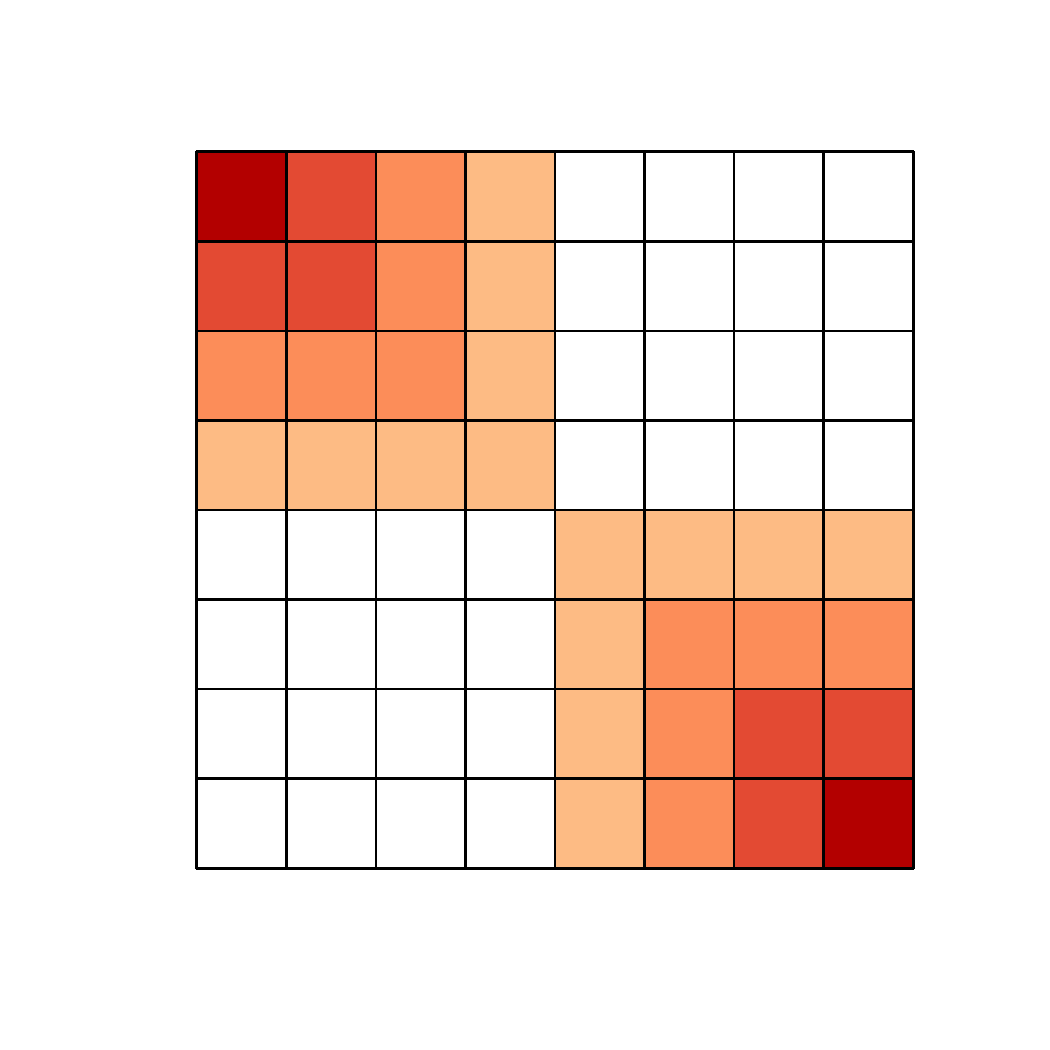
\includegraphics[scale=.21]{figures/spatial_correlation.pdf}
          \end{subfigure} \\
          
          

  \end{figure}
    \end{minipage}

\end{frame}
%----------------------------------------------------------------------%
\begin{frame}[fragile]
\frametitle{Motivation}

 {\it “Everything is related to everything else, but close things are more related than things that are far apart”} (Tobler, 1979).

\bigskip

\begin{itemize}
  \item One of the major differences between standard econometrics and standard spatial econometrics lies, in the fact that, in order to treat spatial data, we need to use two different sets of information.
  \medskip
  \begin{enumerate}
  \item Observed values of the economic variables.
  \medskip
  \item Particular location where those variables are observed and to the various links of proximity between all spatial observations.
  \end{enumerate}
\end{itemize}

\end{frame}


%----------------------------------------------------------------------%
\begin{frame}[fragile]
\frametitle{Spatial Econometrics: Weights Matrix}

\begin{itemize}
  \item At the heart of traditional spatial econometrics is the definition of the {\it weights matrix}:



\begin{align}
W=\left(\begin{array}{cccc}
w_{11} & \dots & \dots & w_{n1}\\
\vdots & w_{ij} &  & \vdots\\
\vdots &  & \ddots & \vdots\\
w_{n_{1}} & \dots & \dots & w_{nn}
\end{array}\right)_{n\times n}
\end{align}

\item with generic element: $w_{ij}=\begin{cases}
1 & if\,j\in N\left(i\right)\\
0 & o.w
\end{cases}$



\item  $N(i)$ being the set of neighbors of location $j$. By convention, the diagonal elements are set to zero, i.e. $w_{ii}=0$. 


\item Quite often the $W$ matrices are standardized to sum to one in each row $w^*_{ij}=\frac{w_{ij}}{\sum_{j=1}^n w_{ij}}$


\end{itemize}

\end{frame}
%----------------------------------------------------------------------%
\section{Spatial Lag Model}
%----------------------------------------------------------------------%
\begin{frame}[fragile]
\frametitle{Spatial Lag Model}
\framesubtitle{Spatial Autoregressive (SAR) Models}

Let's consider the following model:
\bigskip 
\[
y=\lambda Wy+X\beta+u
\]
\medskip
we assume that $W$ is exogenous

\medskip

If $W$ is row standardized:
\medskip
\begin{itemize}
\item Guarantees $|\lambda|<1$ (Anselin, 1982) 
\item $[0,1]$ Weights
\item $Wy$ Average of neighboring values
\item W is no longer symmetric $\sum_{j}w_{ij}\neq\sum_{i}w_{ji}$ (complicates
computation)
\end{itemize}

\end{frame}
%----------------------------------------------------------------------%
\begin{frame}[fragile]
\frametitle{Spatial Lag Model}
\framesubtitle{Maximum Likelihood Estimator}

Note that we can write 
\bigskip 
\[
(I-\lambda W)y=X\beta+u
\]
\bigskip 
\begin{itemize}
\item We can think this model as a way to correct for loss of information coming from spatial dependence.
\bigskip 
\item $(1-\lambda W)y$ is a spatially filtered dependent variable, i.e.,
the effect of spatial autocorrelation taken out
\end{itemize}

\end{frame}
%----------------------------------------------------------------------%
\begin{frame}[fragile]
\frametitle{Spatial Lag Model}

In this case, endogeneity emerges because the spatially lagged value
of y is correlated with the stochastic disturbance. 
\begin{align}
E((Wy)u')\neq 0
\end{align}

Proof.

Note that $y=(I-\lambda W)^{-1}X\beta+(I-\lambda W)^{-1}u$


Then
\begin{align}
E((Wy)u') & =E(W(I-\lambda W)^{-1}X\beta u'+W(I-\lambda W)^{-1}uu') \\
& =W(I-\lambda W)^{-1}X\beta E(u')+W(I-\lambda W)^{-1}E(uu') \\
& =W(I-\lambda W)^{-1}E(uu') \\
& =\sigma^{2}W(I-\lambda W)^{-1}\neq0 
\end{align}

\end{frame}
%----------------------------------------------------------------------%
\subsection{Maximum Likelihood Estimator}
%----------------------------------------------------------------------%
\begin{frame}[fragile]
\frametitle{Spatial Lag Model}
\framesubtitle{Maximum Likelihood Estimator}
\begin{itemize}
\item One solution that emerged in the literature is MLE.
\item We need an extra assumption, i.e.,  $u\sim_{iid}N(0,\sigma^{2}I)$. 
\end{itemize}

\[
y=(I-\lambda W)^{-1}X\beta+(I-\lambda W)^{-1}u
\]

note that

\[
E(y)=(I-\lambda W)^{-1}X\beta+(I-\lambda W)^{-1}u
\]

\[
=(I-\lambda W)^{-1}X\beta+(I-\lambda W)^{-1}E(u)
\]

\[
=(I-\lambda W)^{-1}X\beta
\]


\end{frame}
%----------------------------------------------------------------------%
\begin{frame}[fragile]
\frametitle{Spatial Lag Model}
\framesubtitle{Maximum Likelihood Estimator}



\begin{align}
E(yy') & =((I-\lambda W)^{-1}X\beta+(I-\lambda W)^{-1}u))((I-\lambda W)^{-1}X\beta+(I-\lambda W)^{-1}u)' \nonumber \\ 
& = (I-\lambda W)^{-1}X\beta\beta'X'(I-\lambda W')^{-1}+(I-\lambda W)^{-1}u\beta'X'(I-\lambda W')^{-1} \nonumber \\
&+(I-\lambda W)^{-1}X\beta u'(I-\lambda W')^{-1}+(I-\lambda W)^{-1}uu'(I-\lambda W')^{-1}  \nonumber\\
&=(I-\lambda W)^{-1}X\beta\beta'X'(I-\lambda W')^{-1}+(I-\lambda W)^{-1}uu'(I-\lambda W')^{-1}  \nonumber \\
&=(I-\lambda W)^{-1}X\beta\beta'X'(I-\lambda W')^{-1}+(I-\lambda W)^{-1}(I-\lambda W')^{-1}\sigma^{2} \nonumber 
\end{align}

then

\begin{align}
V(y)&=E(yy')-(E(y))^2 \nonumber \\ 
&=[(I-\lambda W)'(I-\lambda W)]^{-1}\sigma^{2} \nonumber \\ 
&=\Omega\sigma^{2}
\end{align}


\end{frame}
%----------------------------------------------------------------------%
\begin{frame}[fragile]
\frametitle{Spatial Lag Model}
\framesubtitle{Maximum Likelihood Estimator}


The associated likelihood function is then
\begin{scriptsize}
\begin{equation}
\mathcal{L}\left(\sigma^{2},\lambda,y\right)=\left(\frac{1}{\sqrt{2\pi}}\right)^{n}|\sigma^{2}\Omega|^{-\frac{1}{2}}exp\left\{ -\frac{1}{2\sigma^{2}}(y-(I-\lambda W)^{-1}X\beta)'\Omega^{-1}(y-(I-\lambda W)^{-1}X\beta)\right\}  \nonumber
\end{equation}
\end{scriptsize}


the log likelihood

\begin{scriptsize}
\begin{equation}
l\left(\sigma^{2},\lambda,y\right)=constant-\frac{1}{2}ln|\sigma^{2}\Omega|-\frac{1}{2\sigma^{2}}(y-(I-\lambda W)^{-1}X\beta)'\Omega^{-1}(y-(I-\lambda W)^{-1}X\beta) \nonumber
\end{equation}
\end{scriptsize}

note that $|\sigma^{2}\Omega|=\sigma^{2n}|\Omega|$, and that 
\begin{align}
|\Omega| &= |[(I-\lambda W)'(I-\lambda W)]^{-1}| \nonumber \\
&= |(I-\lambda W)^{-1}(I-\lambda W')^{-1}| \nonumber \\
&=|(I-\lambda W)^{-1}||(I-\lambda W')^{-1}| \nonumber \\
&=|(I-\lambda W)|^{-2} \nonumber \\
\end{align}

\end{frame}
%----------------------------------------------------------------------%
\begin{frame}[fragile]
\frametitle{Spatial Lag Model}
\framesubtitle{Maximum Likelihood Estimator}


so returning to the log likelihood we have that  the log likelihood is 

\begin{align}
l\left(\sigma^{2},\lambda,y\right)&=constant-\frac{n}{2}ln\left(\sigma^{2}\right)+ln\left(|(I-\lambda W)|\right) \nonumber \\
&-\frac{1}{2\sigma^{2}}\left(y-(I-\lambda W)^{-1}X\beta\right)'(I-\lambda W)'(I-\lambda W)\left(y-(I-\lambda W)^{-1}X\beta\right)
\end{align}

then 

\begin{align}
l\left(\sigma^{2},\lambda,y\right)&=constant-\frac{n}{2}ln\left(\sigma^{2}\right) \nonumber \\
&-\frac{1}{2\sigma^{2}}\left((I-\lambda W)y-X\beta\right)'\left((I-\lambda W)y-X\beta\right) \nonumber \\
&+ln\left(|(I-\lambda W)|\right)
\end{align}


\end{frame}
%----------------------------------------------------------------------%
\begin{frame}[fragile]
\frametitle{Spatial Lag Model}
\framesubtitle{Maximum Likelihood Estimator}

\begin{itemize}
\item The determinant $|(I-\lambda W)|$ is quite complicated because in contrast to the time series, where it is a triangular matrix, here it is a full matrix. 
\item However, Ord (1975) showed that it can be expressed as a function of the eigenvalues $\omega_{i}$
\end{itemize}


\[
|(I-\lambda W)|=\Pi_{i=1}^{n}(1-\lambda\omega_{i})
\]

So the log likelihood is simplified to 

\begin{align}
l\left(\sigma^{2},\lambda,y\right)&=constant-\frac{n}{2}ln\left(\sigma^{2}\right) \nonumber \\
&-\frac{1}{2\sigma^{2}}((I-\lambda W)y-X\beta)'((I-\lambda W)-X\beta) \nonumber \\
&+\sum ln(1-\lambda\omega_{i})
\end{align}

\end{frame}
%----------------------------------------------------------------------%
\begin{frame}[fragile]
\frametitle{Spatial Lag Model}
\framesubtitle{Maximum Likelihood Estimator}

Applying  FOC, the ML estimates for $\beta$ and $\sigma^{2}$ are:
\bigskip
\[
\hat \beta_{MLE}=(X'X)^{-1}X'(I-\lambda W)y
\]
\bigskip
\[
\hat{\sigma}_{MLE}^{2}=\frac{1}{n}(y-\lambda Xy-X \hat{\beta}_{MLE})'(y-\lambda Xy-X \hat{\beta}_{MLE})
\]

\bigskip
\begin{itemize}
\item Conditional on $\lambda$ these estimates are simply OLS applied to the spatially filtered dependent variable and explanatory variables X.
\end{itemize}


\end{frame}
%----------------------------------------------------------------------%
\begin{frame}[fragile]
\frametitle{Spatial Lag Model}
\framesubtitle{Maximum Likelihood Estimator}
\begin{itemize}
\item  Substituting these in the log likelihood we have a concentrated log-likelihood as a nonlinear function of a single parameter $\lambda$
\end{itemize}
 
 \medskip
\begin{align}
l\left(\lambda\right)=-\frac{n}{2}ln\left(\frac{1}{n}(e_{0}-\lambda e_{L})'(e_{0}-\lambda e_{L})\right)+\sum ln(1-\lambda\omega_{i})
\end{align}
\medskip
\begin{itemize}
\item where $e_{0}$ are the residuals in a regression of $y$ on $X$ and
\item $e_{L}$ of a regression of $Wy$ on $X$. 
\item This expression can be maximized numerically to obtain the estimators for the unknown parameters $\lambda$.
\item with $\lambda^*$, get $\hat \beta_{MLE}$ and  $\hat{\sigma}_{MLE}^{2}$
\end{itemize}



\end{frame}
%----------------------------------------------------------------------%
\begin{frame}[fragile]
\frametitle{Spatial Lag Model}
\framesubtitle{Maximum Likelihood Estimator}
 The asymptotic variance follows as the inverse of the information matrix
\bigskip
\begin{scriptsize}
\begin{align}
AsyVar\left(\lambda,\beta,\sigma^{2}\right)=\left(\begin{array}{ccc}
tr(W_{A})^{2}+tr(W_{A}'W_{A})+\frac{(W_{A}X\beta)'(W_{A}X\beta)}{\sigma^{2}} & \frac{(X'W_{A}X\beta)'}{\sigma^{2}} & \frac{tr(W_{A})'}{\sigma^{2}}\\
\frac{(X'W_{A}X\beta)'}{\sigma^{2}} & \frac{(X'X)}{\sigma^{2}} & 0\\
\frac{tr(W_{A})'}{\sigma^{2}} & 0 & \frac{n}{2\sigma^{4}} 
\end{array}\right)^{-1}
\end{align}
\end{scriptsize}

\bigskip
\begin{itemize}
\item where $W_{A}=W(I-\lambda W)^{-1}$. 
\item Note that 
\begin{itemize}
  \item the covariance between $\beta$ and $\sigma^{2}$ is zero, as in the standard regression model, 
  \item this is not the case for $\lambda$ and $\sigma^{2}.$ 
\end{itemize}

\end{itemize}


\end{frame}
%----------------------------------------------------------------------%
\subsection{Two-Stage Least Squares estimators}
%----------------------------------------------------------------------%
\begin{frame}[fragile]
\frametitle{Spatial Lag Model}
\framesubtitle{Two-Stage Least Squares estimators}

\begin{itemize}
\item An alternative to MLE we can use 2SLS to eliminate endogeneity.
\bigskip
\item Key is to identify proper instruments
\bigskip
\begin{itemize}
\item Need to be uncorrelated with the error term
\bigskip
\item Correlated with $Wy$
\end{itemize}
\end{itemize}

\end{frame}
%----------------------------------------------------------------------%
\begin{frame}[fragile]
\frametitle{Spatial Lag Model}
\framesubtitle{Two-Stage Least Squares estimators}
Consider the following

\[
E(y)=(I-\lambda W)^{-1}X\beta
\]

now, since $|\lambda|<1$ we can use Neumann series property to expand
the inverse matrix as 

\[
(I-\lambda W)^{-1}=I+\lambda W+\lambda^{2}W^{2}+\lambda^{3}W^{3}+....
\]

hence

\[
E(y)=(I+\lambda W+\lambda^{2}W^{2}+\lambda^{3}W^{3}+....)X\beta
\]

\[
=X\beta+\lambda WX\beta+\lambda^{2}W^{2}X\beta+\lambda^{3}W^{3}X\beta+....
\]

so we can express $E(y)$ as a function of $X$, $WX$, $W^{2}X$,... 


\end{frame}
%----------------------------------------------------------------------%
\begin{frame}[fragile]
\frametitle{Spatial Lag Model}
\framesubtitle{Two-Stage Least Squares estimators}

We can use the first three elements of the expansion as instruments.
Let's define $H$ as the matrix with our instruments 

\[
H=[X,WX,W^{2}X]
\]

Now, 

\[
y=\lambda Wy+X\beta+u
\]

\[
=M\theta+u
\]

\medskip
where $M=[Wy,X]$ and $\theta=[\lambda,\beta]$. 

\end{frame}
%----------------------------------------------------------------------%
\begin{frame}[fragile]
\frametitle{Spatial Lag Model}
\framesubtitle{Two-Stage Least Squares estimators}

\begin{itemize}


\item The first stage is: $M=H\gamma+\eta$

\begin{itemize}
  \item where $\hat{\gamma}=(H'H)^{-1}H'M$

  \item and $\hat{M}=H\hat{\gamma}=P_{H}M$
\end{itemize}

\item The second stage is 

\begin{align}
y=\hat{M}\theta+u
\end{align}

and 

\begin{align}
\hat{\theta}_{2SLS}&=(\hat{M}'\hat{M})^{-1}\hat{M}'y \nonumber \\
&=(M'P_{H}M)^{-1}M'P_{H}y
\end{align}

\end{itemize}

\end{frame}
%----------------------------------------------------------------------%
\section{Interpretation of Parameters}
%----------------------------------------------------------------------%
\begin{frame}
\frametitle{Interpretation of Parameters}
\begin{itemize}
  \item Consider the following model for the $i-th$ observation
\begin{align}
y_i = \beta_0 +\beta_1 x_{i1}+\beta_2 x_{i2}+\dots+\beta_r x_{ir}+\dots+\beta_k x_{ik} \,\,\, i=1,\dots,n \nonumber
\end{align}

  \item Recall that in OLS we have


\begin{align}
\beta_1=\frac{\partial y_i}{\partial x_{i1}} \nonumber
\end{align}

or generically
\begin{align}
\beta_r&=\frac{\partial y_i}{\partial x_{ir}}  \,\,\,\,  \forall i=1,\dots,n\,\,\&\,\, r=1,\dots,k \nonumber \\
\beta_r&=\frac{\partial y_i}{\partial x_{jr}} \,\,\,\,  \forall j\neq i\,\,\&\,\, \forall r=1,\dots,k \nonumber
\end{align}

\item Interpretation is straight forward as long as we take into account units
\medskip
\item In spatial models the interpretation is less immediate and require some clarification
\end{itemize}

\end{frame}
%----------------------------------------------------------------------%
\begin{frame}
\frametitle{Interpretation of Parameters}
\begin{itemize}
\item Lets consider the case of a simple Spatial Lag model with a single regressor
\end{itemize}

\begin{align}
y_i = \alpha + \beta x_i + \lambda \sum w_{ij} y_j + \epsilon_i
\end{align}
with $|\lambda|<1$, and 

\begin{align}
\beta \neq \frac{\partial y_i}{\partial x_{i}} \nonumber
\end{align}

\begin{align}
 \frac{\partial y_i}{\partial x_{i}} = diag(I-\lambda W)^{-1}\beta \nonumber
\end{align}
\begin{itemize}
  \item The impact depends also on the parameter $\lambda$
  \item The impact is different in each location
\end{itemize}  


\end{frame}
%----------------------------------------------------------------------%
\begin{frame}
\frametitle{Interpretation of Parameters}
More generally consider 

\begin{align}
y&=\lambda Wy+X\beta+u \nonumber \\
 &=(I-\lambda W)^{-1}X\beta+(I-\lambda W)^{-1}u \nonumber
\end{align}

Then 
\begin{align}
E(y)=(I-\lambda W)^{-1}X\beta
\end{align}

we define

\begin{align}
S(W)=(I-\lambda W)^{-1}\beta
\end{align}
\end{frame}
%----------------------------------------------------------------------%
\begin{frame}
\frametitle{Interpretation of Parameters}
Therefore the impact of {\it each variable}  $x$ on $y$ can be described through the partial derivatives $\frac{\partial E(y)}{\partial x}$ which can be arranged in the following matrix:

\bigskip

\begin{align}
S(W)=\frac{\partial E(y)}{\partial x}=\left(\begin{array}{ccc}
\frac{\partial E(y_{1})}{\partial x_{1}} & \dots & \frac{\partial E(y_{1})}{\partial x_{n}}\\
\vdots & \ddots & \vdots\\
\frac{\partial E(y_{i})}{\partial x_{1}} & \dots & \frac{\partial E(y_{i})}{\partial x_{n}}\\ 
\vdots & \ddots & \vdots\\
\frac{\partial E(y_{n})}{\partial x_{1}} & \dots & \frac{\partial E(y_{n})}{\partial x_{n}}
\end{array}\right)
\end{align}

%then

%\begin{align}
% \frac{\partial E(y_i)}{\partial x_{jr}}=S_r(W)_{ij}
%\end{align}
%and

%\begin{align}
% \frac{\partial E(y_i)}{\partial x_{ir}}=S_r(W)_{ii}
%\end{align}

\end{frame}
%----------------------------------------------------------------------%
\begin{frame}
\frametitle{Interpretation of Parameters}
On this basis, LeSage and Pace (2009) suggested the following impact measures that can be calculated for each independent variable $X_i$ included in the model 

\begin{itemize}
\item {\it Average Direct Impact}: this measure refers to the impact of changes in the $i‐th$ observation of $x$, which we denote $x_{i}$, on $y_i$. This is the average of all diagonal entries in $S$
\end{itemize}

\begin{align}
ADI &= \frac{tr(S(W))}{n} \nonumber \\
&= \frac{1}{n}\sum_{i=1}^n S(W)_{ii}
\end{align}


\end{frame}
%----------------------------------------------------------------------%
\begin{frame}
\frametitle{Interpretation of Parameters}

\begin{itemize}
\item {\it Average Total Impact To} an observation: this measure is related to the impact produced on one single observation $y_i$. For each observation this is calculated as the sum of the $i-th$ row of matrix $S$
\end{itemize}

\begin{align}
ATIT_j &= \frac{\iota'S(W)}{n} \nonumber \\
&= \frac{1}{n}\sum_{i=1}^n S(W)_{ij}
\end{align}


\end{frame}
%----------------------------------------------------------------------%
\begin{frame}
\frametitle{Interpretation of Parameters}

\begin{itemize}
\item {\it Average Total Impact From} an observation: this measure is related to the total impact on all other observations $y_i$ . For each observation this is calculated as the sum of the $j-th$ column of matrix $S$
\end{itemize}

\begin{align}
ATIF_i &= \frac{1}{n}S(W)\iota \nonumber \\
&= \frac{\sum_{j=1}^n S(W)_{ij}}{n} 
\end{align}


\end{frame}
%----------------------------------------------------------------------%
\begin{frame}
\frametitle{Interpretation of Parameters}

\begin{itemize}
\item A Global measure of the average impact obtained from the two previous measures. 
\item It is simply the average of all entries of matrix S
\end{itemize}

\begin{align}
ATI &= \frac{1}{n}\iota'S(W) \iota = \frac{1}{n}\sum_{i=1}^n\ ATIT_i = \frac{1}{n}\sum_{j=1}^n\ ATIF_i
\end{align}

\begin{itemize}
  \item The numerical values of the summary measures for the two forms of average total impacts are equal.
  \item The ATIF relates how changes in a single observation j influences all observations.
  \item In contrast, the ATIT considers how changes in all observations influence a single observation i.
\end{itemize}


\end{frame}
%----------------------------------------------------------------------%
\begin{frame}
\frametitle{Interpretation of Parameters}

\begin{itemize}
\item {\it Average Indirect Impact} obtained as the difference between ATI and ADI
\end{itemize}

\begin{align}
AII = ATI - ADI
\end{align}

\bigskip

\begin{itemize}
\item It is simply the average of all off-diagonal entries of matrix $S$
\end{itemize}


\end{frame}
%----------------------------------------------------------------------%
\begin{frame}
\frametitle{Interpretation of Parameters: Example}
\begin{itemize}
  \item We have data on 20 Italian regions on GDP and unemployment. 
  \item We want to estimate the effect of GDP on Unemployment (Okun's Law)
\end{itemize}


\begin{table}[H]
\begin{tabular}{lcc} \\
[-1.8ex] \hline \hline \\[-1.8ex]
          & OLS       & Spatial Lag Model \\
 \hline \\[-1.8ex]          
Intercept & 10.971*** & 3.12275***        \\
GDP       & ‐3.326*** & ‐1.13532***       \\
$\lambda$ & -         & 0.7476***         \\
ADI       & -         & ‐1.542448         \\
AII       & -         & -2.95571           \\
ATI       & -         & ‐4.498159        \\
\hline \hline \\[-1.8ex]
\end{tabular}
\end{table}

\end{frame}
%----------------------------------------------------------------------%
\begin{frame}
\frametitle{Review \& Next Steps}
  
  \begin{itemize} 
    \item Today:
    \medskip
    \begin{itemize} 
        \item Details on Spatial Lag Model
        \medskip
        \item Interpretation
        \medskip
      \end{itemize}
  	\bigskip  

	\item  Next class: Prediction, prediction, prediction, ...




\end{itemize}
\end{frame}

%----------------------------------------------------------------------%
\section{Further Readings}
%----------------------------------------------------------------------%
\begin{frame}
\frametitle{Further Readings}

\begin{itemize}

   
  \item Arbia, G. (2014). A primer for spatial econometrics with applications in R. Palgrave Macmillan. (Chapter 2 and 3)
  \medskip
  \item Anselin, Luc, \& Anil K Bera. 1998. “Spatial Dependence in Linear Regression Models with an Introduction to Spatial Econometrics.” Statistics Textbooks and Monographs 155. MARCEL DEKKER AG: 237–90.
  \medskip
  \item Anselin, L. (1982). A note on small sample properties of estimators in a first-order spatial autoregressive model. Environment and Planning A, 14(8), 1023-1030.
  \medskip
  \item Tobler, WR. 1979. “Cellular Geography.” In Philosophy in Geography, 379–86. Springer.
\end{itemize}

\end{frame}






%----------------------------------------------------------------------%
%----------------------------------------------------------------------%
\end{document}
%----------------------------------------------------------------------%
%----------------------------------------------------------------------%

